\documentclass[10pt,twocolumn,letterpaper]{article}

\usepackage{cvpr}
\usepackage{times}
\usepackage{epsfig}
\usepackage{graphicx}
\usepackage{amsmath}
\usepackage{amssymb}
\usepackage{enumitem}

% Include other packages here, before hyperref.

% If you comment hyperref and then uncomment it, you should delete
% egpaper.aux before re-running latex.  (Or just hit 'q' on the first latex
% run, let it finish, and you should be clear).
\usepackage[breaklinks=true,bookmarks=false]{hyperref}

\cvprfinalcopy % *** Uncomment this line for the final submission

\def\cvprPaperID{****} % *** Enter the CVPR Paper ID here
\def\httilde{\mbox{\tt\raisebox{-.5ex}{\symbol{126}}}}

% Pages are numbered in submission mode, and unnumbered in camera-ready
%\ifcvprfinal\pagestyle{empty}\fi
\setcounter{page}{1}
\begin{document}

%%%%%%%%% TITLE
\title{Online Knowledge Distillation Methods: A Survey}

\author{Yuan Zhang\\
College of Computer Science, Zhejiang University, China\\
{\tt\small yuan\_zhang@zju.edu.cn}
% For a paper whose authors are all at the same institution,
% omit the following lines up until the closing ``}''.
% Additional authors and addresses can be added with ``\and'',
% just like the second author.
% To save space, use either the email address or home page, not both
% \and
% Second Author\\
% Institution2\\
% First line of institution2 address\\
% {\tt\small secondauthor@i2.org}
}

\maketitle
%\thispagestyle{empty}

%%%%%%%%% ABSTRACT
\begin{abstract}
   Consistency 
\end{abstract}

%%%%%%%%% BODY TEXT
\section{Introduction}
During the last few years, deep learning has gained impressive success
in artificial intelligence. To gain better performance, the deep learning networks
is growing larger and larger. These models have achieved overwhelming
success, however the large size causes heavy computational load during inference. To
deploy such models in real-time applications or on devices with limited resources,
their size should be reduced.

Knowledge distillation~\cite{hinton2015distilling} is one of the methods to reduce
network size with acceptable accuracy drop. It is a process of extracting knowledge
from a complicated teacher network to a simple student network. According to whether teacher is updated simultaneously with student, knowledge distillation methods
are categorized into online methods and offline methods. In offline methods~\cite{liu2019knowledge}~\cite{mirzadeh2020improved}~\cite{passalis2020heterogeneous}~\cite{romero2014fitnets} the teacher networks
are pre-trained and fixed, thus before distillation there is a stage to train the teacher.
Offline methods are simple and fast if the teacher network is provided. However, when the teacher network is not presented,
offline methods begin to expose their limitations:
\begin{enumerate}
   \item Training and tuning a complex teacher network costs a lot of time and effort. And this stage may be performed several times for different tasks or trying different teacher networks.
   \item There is a gap between student and teacher, more specifically, a better teacher does not grant a better student~\cite{mirzadeh2020improved}. This makes researchers wonder whether a group of weak teachers will give better performance.
   \item It is not easy to decide the teacher framework. Usually the teacher network is just a wider version of student network. However, its size cannot be arbitrarily large. As mentioned in second point,
   a wider teacher with better performance may result in a worse student.
 \end{enumerate}

The single-stage online methods are developed to address these problems.
The earliest online methods~\cite{anil2018large}~\cite{zhang2018deep} start from a group of random networks and 
learn from each other during the distillation process. Anil \etal~\cite{anil2018large} employ their method to train
large-scale distributed neural networks and prove online knowledge distillation is a universal and powerful method
to train a simple neural network. Later such methods are developed into ensumble methods~\cite{chen2020online}~\cite{guo2020online}~\cite{lan2018knowledge}, where the student networks learn
from an ensumble of themselves. In~\cite{lan2018knowledge} and~\cite{song2018collaborative} a branch model is used to reduce the memory cost of too many networks.

Some methods are not in the framework of ensumble network.~\cite{yao2020knowledge} appends classifiers to hidden layers so that these layers participate the online distillation process explicitly.
~\cite{chung2020feature} introduces adversarial learning into online distillation.

In this paper some of ensumble online methods are discussed.
Section ~\ref{vanilla_kd} will introduce the original form of knowledge distillation, which is the basis of online knowledge distillation.
Section ~\ref{ensubmle_model} will show most online methods follow
an ensumble framework.
Section ~\ref{review} will review these methods and discuss the challenges and opportunities in online knowledge distillation.
%-------------------------------------------------------------------------
\begin{figure*}
   \begin{center}
   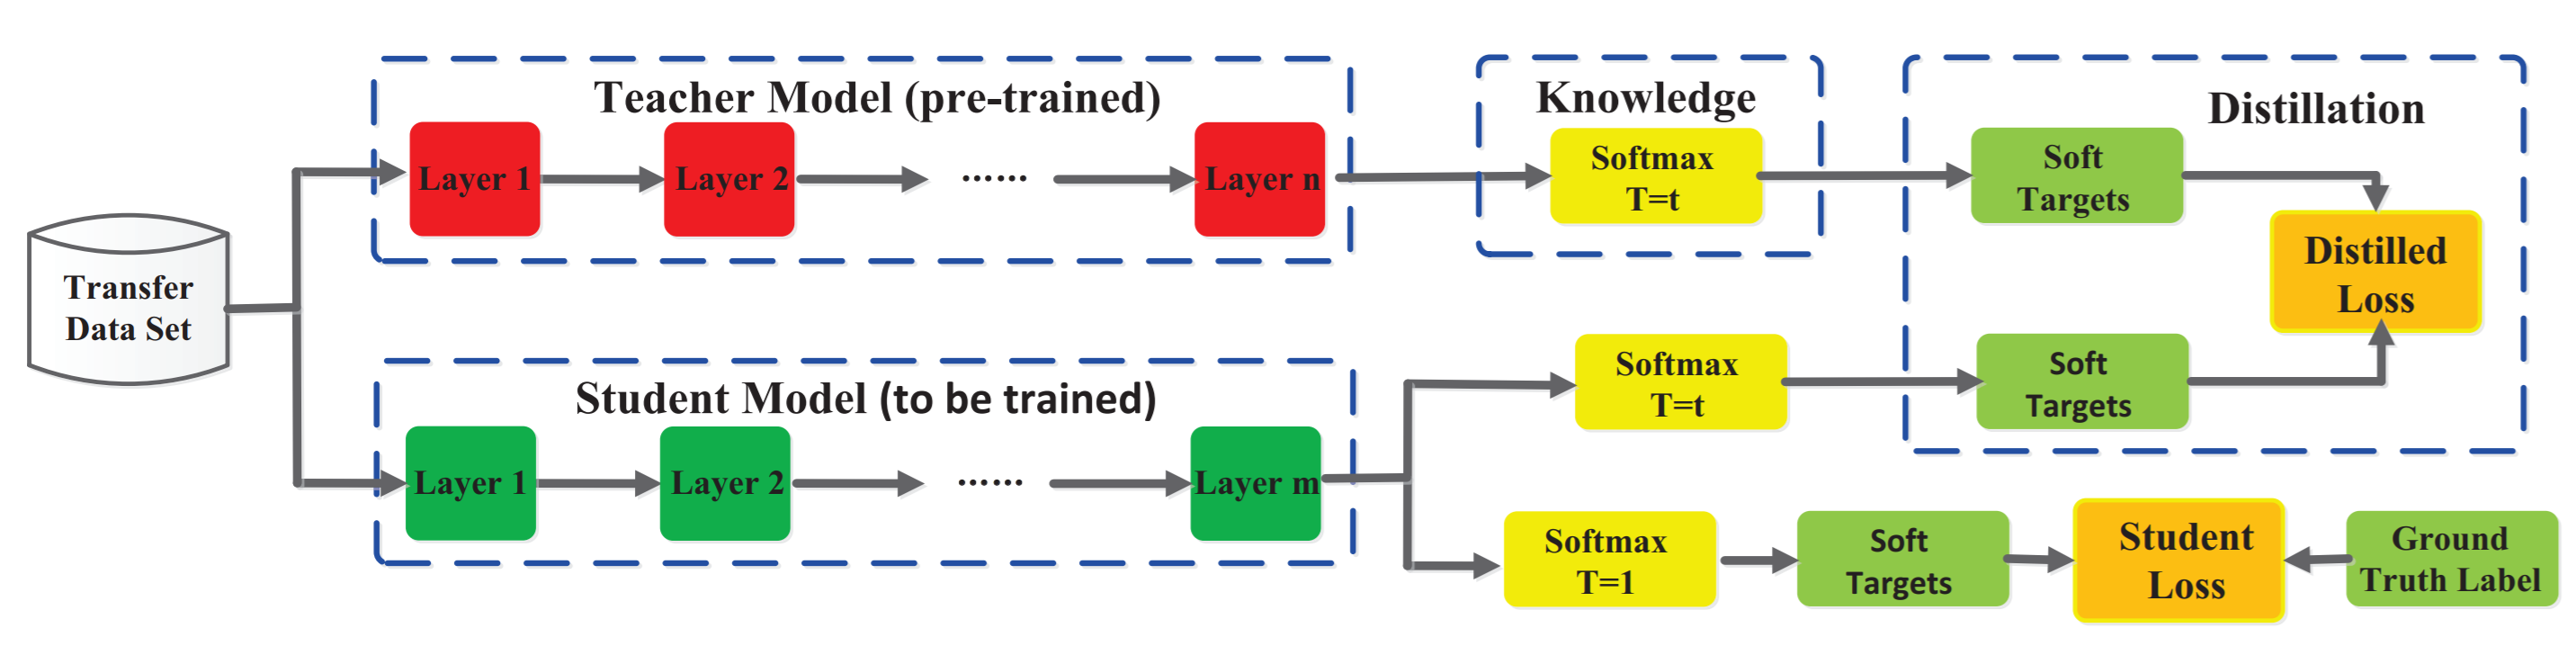
\includegraphics[width=0.9\linewidth]{vanilla_kd.png}
   \end{center}
      \caption{Vanilla Knowledge Distillation}
   \label{fig:vanilla_kd}
\end{figure*}
   
%------------------------------------------------------------------------
\section{Vanilla Knowledge Distillation}\label{vanilla_kd}
Figure~\ref{fig:vanilla_kd} shows the structure of vanilla knowledge distillation. Denote T as the pretrained teacher network and
denote S as the student network to be trained. Two copies of data are sent to T and S respectively.
The knowledge extracted from output of T is used to direct the training of S.

Formally, suppose there is a classification task with a labeled dataset $\mathcal D=\{(x_i, y_i)\}_i^n$, and $f_S(x;\theta):\mathcal X\mapsto\mathbb{R}^m$ is the logits function of the student network S. The parameters of T is fixed
during distillation so that function $f_T(x)$ without parameters is used to denote its logits function.

Equation ~\eqref{eqn:kd_loss} gives the distillation loss, where $\textrm{H}(p, q)$ is cross entroy loss function, $\sigma$ is softmax function and $t$ is temperature of softmax function. Equation ~\eqref{eqn:gt_loss} gives the
ground truth loss of classification. The final training loss is a weighted sum of this two terms.

\begin{equation}
\label{eqn:kd_loss}
   \begin{split}
   L_{\textrm{KD}}(T, S) = \sum\limits_{(x_i, y_i)\in \mathcal D}{\textrm{H}(\sigma(\frac{f_T(x_i)}{t}), \sigma(\frac{f_S(x_i; \theta)}{t}))}
   \end{split}
\end{equation}

\begin{equation}
\label{eqn:gt_loss}
L_{\textrm{GT}}=\sum\limits_{(x_i, y_i)\in \mathcal D}{\textrm{H}(\textrm{one-hot}(y_i),\sigma(f_S(x_i; \theta)))}
\end{equation}

%------------------------------------------------------------------------
\section{Ensumble Model}\label{ensubmle_model}
An ensubmle model will be proposed here. Then the text will explain how most online methods fit in this model.

Suppose a group of student networks $S_1,\dots, S_s$. Now there is no powerful pretrained teacher networks. A group of weighted sums of student logits becomes the teacher logits, as calculated in Equation~\ref{eqn:ensumble}, where
weights $\{w_{ij}; i, j=1,\dots,s\}$ are calculated in different way across different methods. Note that these weights
can be updated, in~\cite{lan2018knowledge} and~\cite{chen2020online}
they are a part of the network, in~\cite{guo2020online} they are calculated after several iterations.

\begin{equation}
\label{eqn:ensumble}
f_{T_i}(x; \Theta) = \sum\limits_{j=1,\dots,s}{w_{ij} f_{S_j}(x; \theta_j)}
\end{equation}

Then these sums are used to teach students in the same way as Equation~\ref{eqn:kd_loss}. The distillation loss is given by Equation~\ref{eqn:ensumble_loss}.
\begin{equation}
\label{eqn:ensumble_loss}
L_{\textrm{ensumble}}=\sum\limits_{i=1,\dots,s}{L_{\textrm{KD}}(T_i, S_i)}
\end{equation}

Also the ground truth loss in Equation~\ref{eqn:gt_loss} for each student is added in the final total loss. Some methods also consider
the ground truth loss for the ensumbles.

Most online methods follow the above framework. In~\cite{lan2018knowledge}, the weights are nodes of the networks and involve the backward process.
In~\cite{chen2020online} they are attentions calculated by the layer before logit layer.~\cite{zhang2018deep} does not strictly fit the framework, it
aggregates difference of each pair of student networks as the knowledge distillation loss. However, it is approximate to the loss from the above framework where each teacher is
an the average of all other student logits.

Here comes the question: How can we get a good group of weights?~\cite{chen2020online} answers this question with attention mechanism~\cite{vaswani2017attention}, letting neural networks learn weights automatically. ~\cite{guo2020online} suppose the best linear
combination of student logits gives good result, and transform this problem to an optimization problem. Yet there is
no powerful theory or practical result to show how to get a better group of weights.


\begin{figure*}
\begin{center}
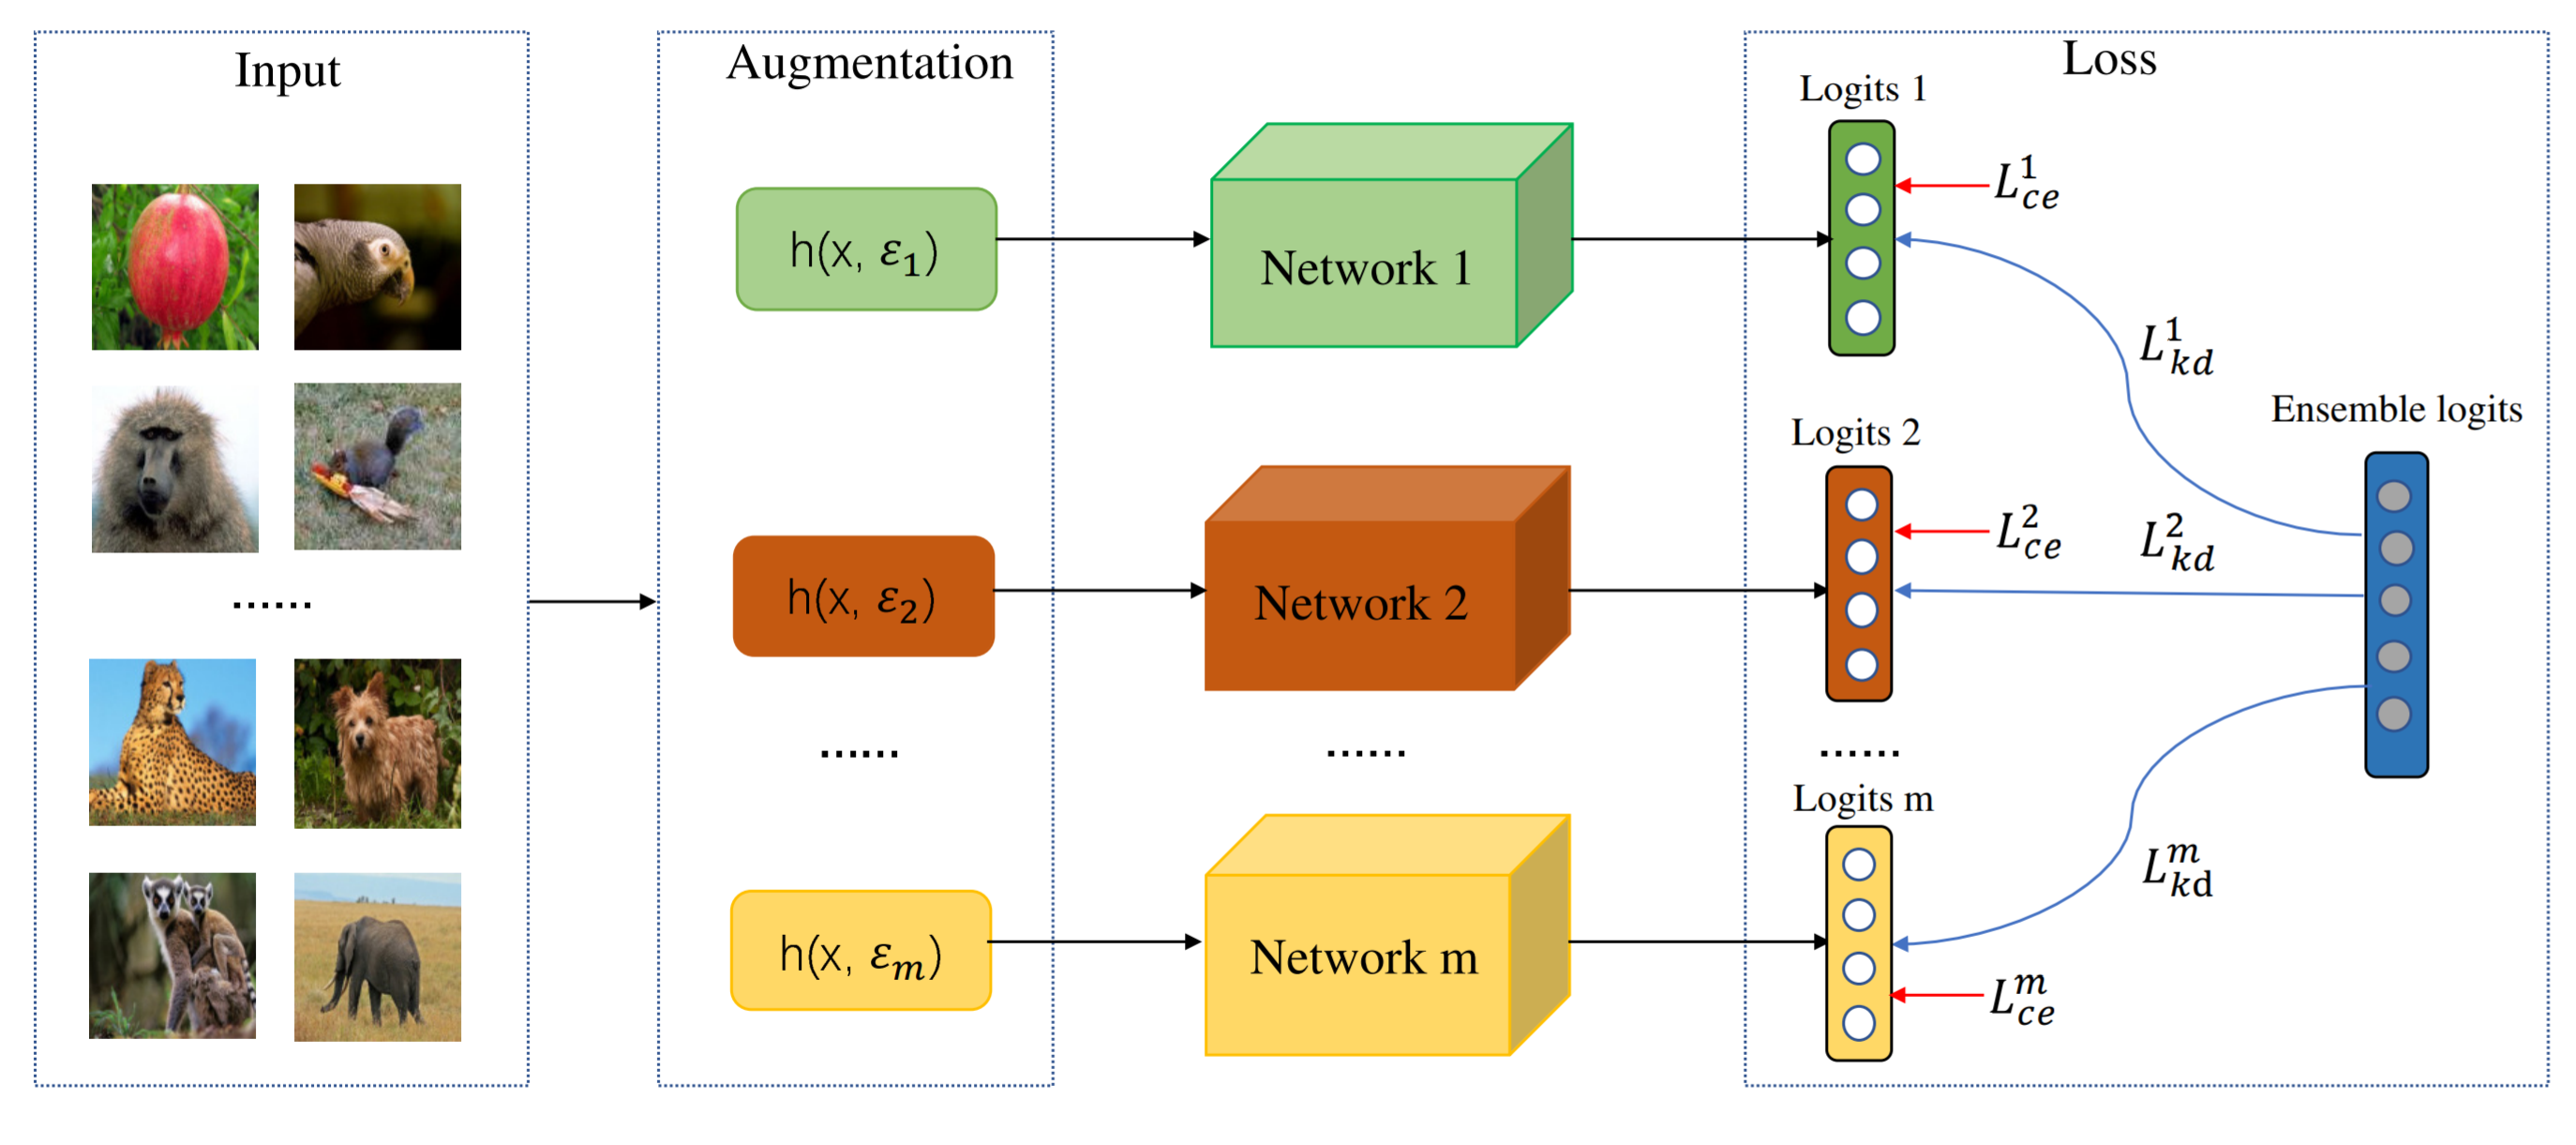
\includegraphics[width=0.9\linewidth]{ensumble_teacher.png}
\end{center}
   \caption{The teacher logits in ensumble model. Different but similar input copies are sent to different student networks. The ensubmle logits come from the output of the student networks. Then they are used as the teacher output for distillation.}
\label{fig:ensumble_teacher}
\end{figure*}

%------------------------------------------------------------------------
\section{Challenges and Opportunities}\label{review}
\subsection{Utilization of Hidden Layers} Note that inner layers can be a part the knowledge to distill.
Although more and more offline methods are utilizing knowledge from hidden layers, online methods hardly use this information.
The challenge to use inner layers is that
only same layers across networks can be ensumbled.
Offline methods use FC, CNN, or attention to match layers~\cite{romero2014fitnets}~\cite{yao2020knowledge}~\cite{DBLP:journals/corr/ZagoruykoK16a}~\cite{chen2021cross}.
Online method in~\cite{yao2020knowledge} add classifiers to hidden layers and align output size,
but it is both time consuming and space consuming.
\subcetion{Space Consumption}
space: branch/tree model -> DAG model
explore the capacity of a network structure.
%------------------------------------------------------------------------
\section{Conclusion}
conetent


{\small
\bibliographystyle{ieee_fullname}
\bibliography{a}
}

\end{document}
